\documentclass[times, utf8, zavrsni, english]{fer}
\usepackage{booktabs}
\usepackage[utf8]{inputenc}
\usepackage[T1]{fontenc} 
\usepackage[english]{babel}
\usepackage{natbib}
\bibliographystyle{abbrvnat}
\usepackage{multirow}
\usepackage{graphicx}
\graphicspath{ {./images/} }

\begin{document}


\thesisnumber{596}


\title{Application of machine learning to threat classification from cybersecurity records}


\author{Mirta Medak}

\maketitle

% Dodavanje zahvale ili prazne stranice. Ako ne želite dodati zahvalu, naredbu ostavite radi prazne stranice.
\zahvala{}

\tableofcontents

\chapter{Introduction}
Every entity that is dependent on a computer system, from corporations to individuals, could be a subject to cyberattacks. In 2020, it is approximated that cybercrime costed the global economy almost USD 1 trillion \citep{cremer}. \\
As technology evolves, more various threats to its security emerge.
Tracking, describing, and evaluating these threats is of use when developing defense systems and making business decisions. \\
A \textbf{vulnerability} is a weakness in a computer system that an attacker can exploit to execute malicious commands, access data in an unauthorized way, or perform other types of cyber attacks \citep{humayun}. \\
A \textbf{threat} is any circumstance or event which has the potential to compromise system security \citep{FER}. \\
In order to tackle the cybersecurity problems in a more organized manner, a system of \emph{Common Vulnerability and Exposure} (CVE) has been developed. The MITRE Corporation maintains a public database of an increasing number of CVE records.
A CVE record includes an ID, a brief description of the vulnerability, and references.
In order to manipulate and prioritize vulnerabilities in a system, the metric of the \emph{Common Vulnerability Scoring System} (CVSS) score is used. This metric estimates how "dangerous" exploitation of a vulnerability is. CVSS is an emerging standard of vulnerability comparison \citep{khazaei}. \\
The CVSS score is computed using metrics with descrete values that are assigned by experts. The weight of each metric is hard-coded into a formula \citep{bozorgi}. Khazaei et al. show an important concern in their work: the CVSS calculation \textbf{can be subjective} \citep{khazaei}.
Moreover, the annotation requires experts and time, which prolongs the process and is costly.
Sometimes, the computation of the CVSS score is not possible because some metrics are missing. Many vulnerabilities aren't assigned the score at all \citep{vulnerwatch}.\\

\noindent The main subject of this research is predicting the CVSS score by analyzing the description of the vulnerability, taken from CVE records. This would be a more consistent approach, and the process of obtaining the score would be cheaper and faster. \\
BERT classification model has proven to be 90-95 \% accurate in predicting the CVSS metrics using the description of the vulnerability. \\
BERT is computationally expensive, and sometimes it is advised to try simpler models first, because they might work just as well. That is why Support Vector Regression and similar models were used to predict the score directly from the description.\\

\noindent In the second chapter, the studies with similar concerns are mentioned. The details about the dataset used are explained in the third chapter. The simplified theory behind the models used is shown in the fourth chapter. The following are the explanations of the experiments, together with the results and their comparisons. 

\chapter{Related work}
Inspiration to do this research has been given by the study of Janamian et al., 2021, who have developed an application that takes any vulnerability description and gives its CVSS score. They used BERT classification to predict the Base score submetrics. The CVSS score was then calculated using the hard-coded CVSS formula and the predicted submetrics results. They have achieved accuracy in the 0.90 range. Using the predicted submetrics, they computed the CVSS score using the CVSS formula, and got the result of R2 = 0.505.\\

\noindent Another study developing an objective method of CVSS score calculationused Support Vector Machine, Random-Forest, and fuzzy system \citep{khazaei}. Their model's accuracy was around 0.86. \\

\noindent This problem was approached in detail by Bozorgi et al., 2010.  Instead of predicting the CVSS score itself, they have developed a new classification system, using various features of the vulnerability. \\

\chapter{Data}
\section{Data acquisition}
Dataset used has been acquired and prepared by Janamian et al., when used in their work \emph{Using NLP to Predict the Severity of Cybersecurity Vulnerabilities, 2021.} \citep{vulnerwatch}.
Most of the data is publicly available and maintained by the MITRE organization and the US National Institute of Standards of Technology. \\
From the cited research, we find out that at the beginning of 2021, only 50 \% of CVE records had a CVSS score assigned. \\
The datasets were created by human experts and therefore didn't require much preparation or preprocessing. 

\section{Dataset structure}
The entire dataset counts 77,020 entries. It is split into training set (80\%) and test set (20\%).

\begin{table}[h!]
	\centering
	\begin{tabular}{||c c c ||} 
		\hline
		 & Column Title & Values  \\ [0.5ex] 
		\hline\hline
		
		1 & attack\_vector & physical; adj\_network;   \\
		 & &  local; network \\
		2 & attack\_complexity & high; low  \\
		3 & privileges\_required & high; low; none  \\
		4 & user\_interaction & none; required \\ 
		5 & scope & unchanged; changed \\ 
		6 & confidentiality & high; low; none  \\
		7 & integrity & high; low; none  \\
		8 & availability & high; low; none  \\
		
		\hline\hline
		9 & description & natural language description \\
		10 & base\_score & float from 0 - 10 \\
		\hline
	\end{tabular}
\caption{Columns and their values used in experiments}
\label{table:1}
\end{table}

\noindent The first eight entries of Table 3.1. correspond to eight submetrics of CVSS base score.
The description is used as input in all performed experiments.
The base\_score is a subgroup of CVSS score, which is most widely used when describing the severity of the vulnerability.

\section{Dataset analysis}
According to CVSS v3.0 Ratings the severity is classified in the following ranges.\footnote{\url{https://nvd.nist.gov/vuln-metrics/cvss}}
\begin{table}[h!]
	\centering
	\begin{tabular}{| c c c |} 
		\hline
		Severity & Base score range & No. of examples\\ [0.5ex] 
		\hline\hline
		
		None & 0.0 & 0  \\
		Low &  0.1-3.9 & 1115 \\
		Medium & 4.0-6.9 & 24232  \\
		High & 7.0-8.9  & 26793 \\
		Critical & 9.0-10.0 & 9476\\
		\hline
	\end{tabular}
	\caption{CVSS range classification and number of examples in each class (from the training set)}
	\label{table:2}
\end{table}

\noindent From Table 3.2. we can clearly see that the medium to high scores prevail in the training set.


\begin{table}[h!]
	\centering
	\begin{tabular}{| c | c |} 
		\hline
		Column Title & Values  \\ [0.5ex] 
		\hline\hline
		
		Attack Vector & local  \\
		Attack Complexity & low  \\
		Privileges Required & none  \\
		User Interaction & none; required \\ 
		Scope & unchanged \\ 
		Confidentiality & none  \\
		Integrity & none  \\
		Availability & high  \\
		
		\hline\hline
		
		Base Score & 5.5 \\
		\hline
	\end{tabular}
	\caption{An example of a dataset entry}
	\label{table:3}
\end{table}
\noindent The description of the shown entry: \\
\textit{The JPEGSetupEncode function in tiff\_jpeg.c in LibTIFF 4.0.7 allows remote attackers to cause a denial of service (divide-by-zero error and application crash) via a crafted image.}
An example of a dataset entry can be seen in the Table 3.3. Only the columns used in the experiments are shown. 
\chapter{Models}

\section{Support Vector Regression}
\subsection{Support Vector Machines}
The Support Vector Machine (SVM) was developed in its present form at AT\&T Bell Laboratories by Vapnik et al. \citep{boser}, \citep{smola}. \\
The SVM is a supervised learning model that can be applied to classification, regression, and outliers detection problems. \footnote{\url{https://scikit-learn.org/stable/modules/generated/sklearn.svm.SVR.html}} \\
In classification problems, the output is a discrete variable, and in regression it is continuous. \\

\begin{figure}[h!]
	\centering
	\includegraphics[scale = 0.5]{svm-visualization}
	\caption{Support Vector Regression visualization}
\end{figure}

\noindent The following explanation is taken from the \citep{Awad2015}.
The SV algorithm needs to find a function in n-dimensional space which fits the data. This function is called hyperplane.
Support Vectors are the data points around this function. As shown in the Figure 4.1, a tube is formed symmetrically around the function so that the absolute values of errors less than epsilon are ignored both above and below the estimate. This way, the data points outside of the tube are penalized, and those on the inside are not.
The SVR tries to find the narrowest tube centered around the function while minimizing the prediction error.  \\

\noindent The advantage of SVR is that its complexity does not depend on the dimension of the input space. \\

\noindent Depending on the choice of kernel, data is mapped into different dimensional spaces. Kernel functions can be linear, radial basis function (rbf), polynomial, and sigmoid. \\
The free parameters of the model are C and epsilon. \\
The model is defined by its hyperparameters. They control the way the model fits the data. Their fine-tuning was performed using Bayesian optimization, which is based on the Bayesian theorem. Cross-validation is performed over parameter combinations. More commonly used Grid Search tries out all given combinations of parameters. Bayes Search, as opposed to Grid Search, memorizes the result of the previous combination and uses it to choose the next combination, so that it comes to the optimum more quickly. \citep{WU201926} \\

\noindent The SVR, as well as other Support Vector models that will be mentioned, are implemented using \texttt{scikit-learn} library. Implementation details are described in Chapter 5. Experiments and Results.

\subsection{word2vec}
Word2vec is a way to represent natural language as vectors. It was developed by Mikolov et al. in 2013 \citep{mikolov}. \\
It consists of two learning models: Continuous Bag of Words (CBOW) and Skip-gram. CBOW predicts the word given its context, and Skip-gram predicts the context given a word. \citep{ma} \\
Knowing the distances between vectors, it is possible to group similar words.
This algorithm is used to convert the text input into vectors, after which they can be used in regression and classification tasks using the SVM model.
\subsection{LinearSVR and SGDRegressor}
LinearSVR is similar to a Support Vector Regression model with a linear kernel. 
The difference is that LinearSVR is implemented as a liblinear model, and SVR as libsvm. \footnote{\url{https://scikit-learn.org/stable/modules/generated/sklearn.svm.LinearSVR.html#sklearn.svm.LinearSVR}} \\
SGD stands for Stochastic Gradient Descent. This is an iterative method of finding a function optimum. The gradient of the loss is estimated each sample at a time and the model is updated along the way with a decreasing learning rate. \footnote{\url{https://scikit-learn.org/stable/modules/generated/sklearn.linear_model.SGDRegressor.html#sklearn.linear_model.SGDRegressor}} \\
It is advised to use LinearSVR or SGDRegressor over SVR for large datasets. \footnote{\url{https://scikit-learn.org/stable/modules/generated/sklearn.svm.SVR.html}}

\section{BERT}
\subsection{BERT architecture}
\textbf{Bidirectional Encoder Representations from Transformers} is a fairly new and revolutionary language representation model, developed by Google \citep{47751} \\
BERT is fundamentally a transformer language model.
Developed by Vaswani et al., 2017, the \textbf{Transformer} is a network architecture based on attention mechanisms. Until the invention of transformers, more complicated models such as recurrent and convolutional neural networks with an encoder and a decoder were used to solve translation tasks. The new model improved translation, sequence modeling, and other similar tasks \citep{vaswani}. \\
The transformer architecture is based on an encoder that maps an input to a continuous representation, and a decoder that produces the output using the encoded representation, one element at a time. At every step, the model takes into account the previously encoded symbols by including them in the input. This way, the model considers the context \citep{vaswani}. \\
By definition, an attention function is mapping vectors as a weighted sum to an output, where the vectors correspond to a query, keys, and values. \\
The novelty in the BERT model is the bidirectional encoder, that is, the incorporation of context from both directions. This matters significantly in token-level tasks, such as question answering, token classification, etc. In order to perform bidirectional pre-training, BERT uses masked language models \citep{47751}. \\
A great advantage of BERT over other language models is that the model has been already pre-trained on large text corpora. This model can then be fine-tuned with only one more output layer, and this model can be applied to a variety of tasks \citep{47751}. This framework is called transfer learning. \\
When using BERT for a specific task, we can use an already pre-trained model. Our task is then to fine-tune it.
Fine-tuning is in fact putting data through a transformer self-attention mechanism while optimizing the weights of the model.
\subsection{Data prepartion for BERT}
The dataset has to be split into train, development, and test set.\\
Attributes that are necessary to fine-tune BERT are the following:
\begin{itemize}
	\item input ids - list of tokens, smallest units of text that make sense,
	\item  input mask - implies that all sequences that are longer than a specified length of a sequence will be truncated to that specified length, and those that are shorter will be padded with additional tokens and
	\item label id - id of the label for a sequence.
\end{itemize}
 
\subsection{BERT classification}
As previously mentioned, in order to fine-tune BERT for a specific task, an additional task-related output layer is added to an already pre-trained model.\\
In this research, the \texttt{bert-base-uncased} was used as the pre-trained model.\\
Some common tasks are implemented in the transformers library as the top layer. One of those is BertForSequenceClassification, which was used in this research to predict the eight submetrics of the Base score. 
\subsection{BERT for regression}
Similarly to the classification task, on top of 12 transformers lies a BertRegressor layer that gives the output for a regression task. The Bert Regressor was used to predict the base score directly from the description.\\
BERT Regressor is widely used in machine translation evaluation tasks. \citep{shimanaka}

\chapter{Experiments and results}
\section{Base score prediction from vulnerability description}
The goal of this experiment was to find out if it is possible to accurately obtain the CVSS score by direct analysis of the vulnerability description.
\subsection{Support Vector Regression + word2vec}
The dataset of over 61k entries is too large for the Support Vector Regression model implemented as \texttt{libsvm}, because the fit complexity is more than quadratic with the number of samples.\\
That is why SVR used approximately half of the training data, 30k samples, and 6k test samples. 
10k samples were used to fine-tune the hyperparameters. \\
All samples taken from the initial dataset were stratified with regard to the Base score, that is, the data was chosen in such a way, that the Base score values follow a uniform distribution.\\
Vulnerability description tokens are transformed into vectors and then summarized in order to map one vector to one description.
These vectors are then scaled using the StandardScaler's function \texttt{fit\_transform}, which first fits the input data to the output feature, and then scales it.\\
Parameter fine-tuning is then performed by BayesSearchCV, the function from \texttt{skopt} library. The kernel was set to rbf, because the SVR linear kernel is too slow for large datasets.\\
The optimized hyperparameters are shown in Table 5.1.
\begin{table}[h!]
	\centering
	\begin{tabular}{|| c | c ||} 
		\hline
		Parameter & Value \\ [0.5ex] 
		\hline\hline
		C & 31.6668  \\ \hline
		epsilon & 0.732095 \\ \hline
		tol & 0.003125  \\ 
		\hline
	\end{tabular}
	\caption{Hyperparameteres for SVR}
	\label{table:4}
\end{table}

\begin{table}

	\centering
	\begin{tabular}{|| c | c ||} 
		\hline
		Metric & Value \\ [0.5ex] 
		\hline\hline
		Mean Squared Error & 1.711  \\ \hline
		Explained Variance Score & 0.504\\ \hline
		Maximum Residual Error & 6.186 \\ \hline
		Mean Absolute Percentage Error & 0.167 \\ \hline
		Coefficient of Determination (\textbf{R2 Score}) & \textbf{0.503} \\
		\hline
	\end{tabular}
	\caption{SVR results}
	\label{table:5}

\end{table}

In Table 5.2., the results of the SVR model are shown.
The coefficient of determination is the score of correlation between two values. Its maximum value is 1, which shows the perfect correlation.
The obtained result shows medium level of correlation.

\subsection{Linear Support Vector Regression}
Linear SVR used the entire dataset. The BayesSearchCV was used to optimize the hyperparameters.\\
Because the number of samples was greater than the number of features, the loss function had to be set as \texttt{squared\_epsilon\_insensitive}.
\begin{table}[h!]
	
		\centering
		\begin{tabular}{|| c | c ||} 
			\hline
			Parameter & Value \\ [0.5ex] 
			\hline\hline
			C & 0.065189  \\ \hline
			epsilon & 2.1582e-06 \\ \hline
			tol & 0.00015387  \\ 
			\hline
		\end{tabular}
		\caption{Hyperparameteres for LinearSVR}
		\label{table:6}
\end{table}
\begin{table}
		\centering
		\begin{tabular}{|| c | c ||} 
			\hline
			Metric & Value \\ [0.5ex] 
			\hline\hline
			Mean Squared Error & 1.888  \\ \hline
			Explained Variance Score & 0.302\\ \hline
			Maximum Residual Error & 9.786 \\ \hline
			Mean Absolute Percentage Error & 0.169 \\ \hline
			Coefficient of Determination (\textbf{R2 Score}) & \textbf{0.302} \\
			\hline
		\end{tabular}
		\caption{LinearSVR results}
		\label{table:7}
	
\end{table}

In Table 5.4, we see worse results obtained by Linear Support Vector Regression.
The Maximum Residual Error is almost as large as the range of the base score, which suggests that this model should not be used to predict the score.

\subsection{Stochastic Gradient Descent Regressor}
SGDRegressor used the entire dataset. Bayes Search optimized the hyperparameteres.
\begin{table}[h!]

		\centering
		\begin{tabular}{|| c | c ||} 
			\hline
			Parameter & Value \\ [0.5ex] 
			\hline\hline
			alpha & 5.1431e-05  \\ \hline
			epsilon & 0.37136 \\ \hline
			loss & "huber" \\ \hline
			tol & 1.5939e-07  \\ 
			\hline
		\end{tabular}
		\caption{Hyperparameteres for SGDRegressor}
		\label{table:8}
\end{table}
\begin{table} [h!]
		\centering
		\begin{tabular}{|| c | c ||} 
			\hline
			Metric & Value \\ [0.5ex] 
			\hline\hline
			Mean Squared Error & 1.952  \\ \hline
			Explained Variance Score & 0.279\\ \hline
			Maximum Residual Error & 9.786 \\ \hline
			Mean Absolute Percentage Error & 0.169 \\ \hline
			Coefficient of Determination (\textbf{R2 Score}) & \textbf{0.278} \\
			\hline
		\end{tabular}
		\caption{SGDRegressor results}
		\label{table:9}
\end{table}

In Table 5.6, we see that SGD Regressor similarly failed, with the coefficient of determination of only 0.278.

\subsection{BERT Regressor}
The BERT fine-tuning was done with PyTorch. The library \texttt{transformers} is used to import the tokenizer and \texttt{BertModel} in order to create a class \texttt{BertRegressor}.
Firstly, the descriptions are tokenized using \texttt{BertTokenizer}. Then, the longest description is found. Using the method \texttt{tokenizer.encode\_plus()}, \texttt{input\_ids} and \texttt{attention\_masks} lists are created. Those lists, as well as the labels list, are converted into tensors. \\
The training dataset is split into 80-20 train-validation sets. \\
The optimizer used is AdamW with default parameters, and the scheduler is obtained with the function get\_linear\_schedule\_with\_warmup. 
The loss function is MSELoss.\\
The model was trained for three epochs. 

\begin{table}[h!]
		\centering
		\begin{tabular}{|| c | c ||} 
			\hline
			Metric & Value \\ [0.5ex] 
			\hline\hline
			Mean Squared Error & 1.186  \\ \hline
			Explained Variance Score & 0.563\\ \hline
			Maximum Residual Error & 6.953 \\ \hline
			Mean Absolute Percentage Error & 0.116 \\ \hline
			Coefficient of Determination (\textbf{R2 Score}) & \textbf{0.561} \\
			\hline
		\end{tabular}
		\caption{BERT regressor results}
		\label{table:10}
\end{table}
\subsection{Results comparison}
\begin{table}[h!]
	\centering
	\begin{tabular}{|| c | c ||} 
		\hline
		Model & R2 score \\ [0.5ex] 
		\hline\hline
		SVR & 0.503  \\ \hline
		LinearSVR & 0.302 \\ \hline
		SGDRegressor & 0.278 \\ \hline
		\textbf{BERT Regressor} & \textbf{0.561} \\ 
	
		\hline
	\end{tabular}
	\caption{Models comparison}
	\label{table:11}
\end{table}

In the Table 5.8, we see that BERT Regressor performed better than any other model, but only by a small margin compared to SVR.

\section{Base score metrics classification}
The goal of this experiment was to discover at what level of accuracy can we predict the metrics of the Base score, having the vulnerability description as the input.
\subsection{Baseline}
The Support Vector Classifier with default parameters was used as a baseline model for this prediction.\\
The description tokens were converted into vectors, and the vectors were summarized just like in SVR.

\begin{table}[h!]
	\centering
	\resizebox{\textwidth}{!}{%
	\begin{tabular}{| c | c | c | c | c | c | c |} 
		\hline
		Score Metric & Value & precision & recall & f1-score & support & accuracy \\ [0.5ex] 
		\hline\hline
		\multirow{4}{*}{Attack Vector} & ADJACENT NETWORK & 0.00 & 0.00 & 0.00 & 338 & \multirow{4}{*}{0.82} \\ 
										& LOCAL & 0.84 & 0.46 & 0.60 & 3625 & \\ 
										& NETWORK & 0.82 & 0.98 & 0.89 & 11252 & \\ 
										& PHYSICAL & 0.00 & 0.00 & 0.00 & 189 & \\ 
		\hline
		\multirow{2}{*}{Attack Complexity} & HIGH & 0.94 & 0.33 & 0.49 & 1268 & \multirow{2}{*}{0.94} \\ 
											& LOW & 0.94 & 1.00 & 0.97 & 14136 & \\ 
		\hline
		\multirow{3}{*}{Privileges Required} & HIGH & 0.87 & 0.27 & 0.41 & 1024 & \multirow{3}{*}{0.82} \\ 
											& LOW & 0.77 & 0.63 & 0.69 & 4091 & \\ 
											& NONE & 0.84 & 0.96 & 0.89 & 10289 & \\ 
		\hline
		\multirow{2}{*}{User Interaction} & NONE & 0.90 & 0.96 & 0.93 & 9779 & \multirow{2}{*}{0.91} \\ 
										& REQUIRED & 0.94 & 1.00 & 0.97 & 5634 & \\ 
		\hline
		\multirow{2}{*}{Scope} & CHANGED & 0.97 & 0.77 & 0.86 & 2611 & \multirow{2}{*}{0.96} \\ 
											& UNCHANGED & 0.96 & 1.00 & 0.97 & 12793 & \\ 
		\hline
		\multirow{3}{*}{Confidentiality} & HIGH & 0.81 & 0.96 & 0.88 & 9095 & \multirow{3}{*}{0.84} \\ 
											& LOW & 0.93 & 0.68 & 0.78 & 2957 & \\ 
											& NONE & 0.88 & 0.65 & 0.74 & 3352 & \\ 
		\hline
		\multirow{3}{*}{Integrity} & HIGH & 0.83 & 0.92 & 0.87 & 7895 & \multirow{3}{*}{0.85} \\ 
									& LOW & 0.95 & 0.77 & 0.85 & 2693 & \\ 
									& NONE & 0.85 & 0.79 & 0.82 & 4816 & \\ 
		\hline
		\multirow{3}{*}{Availability} & HIGH & 0.88 & 0.92 & 0.90 & 8994 & \multirow{3}{*}{0.88} \\ 
		& LOW & 0.88 & 0.27 & 0.42 & 413 & \\ 
		& NONE & 0.87 & 0.85 & 0.86 & 5997 & \\ 
		\hline
		
	\end{tabular}}
	\caption{Baseline results}
	\label{table:12}
\end{table}

In Table 5.9, the results of the Support Vector Classifier results are shown. 

Precision metric is accuracy of positive predictions. Recall is the ability of a model to find all positive instances. F1 score is a weighted harmonic mean of precision and recall. The best f1 score is 1.0, and the worst is 0.0. Support is the number of examples of the corresponding value in the tranining dataset.
The accuracy of the model is the percentage of correctly predicted values. \\

For some values, all the metrics are equal to 0.00. This can happen when there is too little data for the classifier to evaluate its performance. Also, it is noticeable that the accuracy of the model is overall higher in the submetrics with only two values, even when the dataset is not balanced.


\subsection{BERT Classification}
The fine-tuning was performed with PyTorch.
Firstly, the dataset was divided into a test set (20\%) and the rest set, which was divided into a training set (80\%) and a development set.\\
From the \texttt{transformers} library, BertForSequenceClassification made up the top layer of the BERT model.\\
In the function convert\_examples\_to\_inputs\textit{(X, y, label2idx, max\_seq\_len, tokenizer)}, a list of token ids, segment ids, and input mask lists were created. Longer descriptions than max\_seq\_len were truncated, while the shorter ones were padded. \\
Usually, batch size is 16 or 32, in this model the value of batch size is 16.
The AdamW optimizer with a base learning rate of 5e-5  is used. The WarmupLinearScheduler linearly increases the learning rate during the warmup stage. During the training, the learning rate slowly decreases again.\\
The model was trained for three epochs.
At each epoch, the model is trained on the training set and evaluated on the development set. \\
To perform the final evaluation, the model is given test data that has never been seen before, and it predicts the metric values. \\

\begin{table}[h!]
	\resizebox{\textwidth}{!}{%
	\centering
	\begin{tabular}{| c | c | c | c | c | c | c |} 
		\hline
		Score Metric & Value & precision & recall & f1-score & support & accuracy \\ [0.5ex] 
		\hline\hline
		\multirow{4}{*}{Attack Vector} & ADJACENT NETWORK & 0.84 & 0.46 & 0.60 & 3625 & \multirow{4}{*}{0.92} \\ 
		& NETWORK & 0.94 & 0.97 & 0.95 & 11267 &
		 \\ 
		& LOCAL & 0.89 & 0.84 & 0.86 & 3632 & \\ 
		& PHYSICAL & 0.83 & 0.67 & 0.74 & 178 & \\ 
		\hline
		\multirow{2}{*}{Attack Complexity} & HIGH & 0.80 & 0.55 & 0.65 & 1234 & \multirow{2}{*}{0.95} \\ 
		& LOW & 0.96 & 0.99 & 0.97 & 14170 & \\ 
		\hline
		\multirow{3}{*}{Privileges Required} & NONE & 0.91 & 0.94 & 0.92 & 10302 & \multirow{3}{*}{0.88} \\ 
		& LOW & 0.81 & 0.78 & 0.80 & 4095 & \\ 
		& HIGH & 0.83 & 0.60 & 0.70 & 1007 & \\ 
		\hline
		\multirow{2}{*}{User Interaction} & NONE & 0.94 & 0.96 & 0.95 & 9932 & \multirow{2}{*}{0.94} \\ 
		& REQUIRED & 0.93 & 0.89 & 0.91 & 5472 & \\ 
		\hline
		\multirow{2}{*}{Scope} & CHANGED & 0.95 & 0.83 & 0.89 & 2556 & \multirow{2}{*}{0.97} \\ 
		& UNCHANGED & 0.97 & 0.99 & 0.98 & 12848 & \\ 
		\hline
		\multirow{3}{*}{Confidentiality} & HIGH & 0.89 & 0.93 & 0.91 & 9069 & \multirow{3}{*}{0.88} \\ 
		& LOW & 0.88 & 0.78 & 0.83 & 2980 & \\ 
		& NONE & 0.86 & 0.84 & 0.85 & 3355 & \\ 
		\hline
		\multirow{3}{*}{Integrity} & HIGH & 0.90 & 0.92 & 0.91 & 7860 & \multirow{3}{*}{0.90} \\ 
		& LOW & 0.92 & 0.82 & 0.87 & 2737 & \\ 
		& NONE & 0.89 & 0.90 & 0.89 & 4807 & \\ 
		\hline
		\multirow{3}{*}{Availability} & HIGH & 0.92 & 0.93 & 0.93 & 8984 & \multirow{3}{*}{0.91} \\ 
		& LOW & 0.76 & 0.32 & 0.45 & 407 & \\ 
		& NONE & 0.89 & 0.92 & 0.90 & 6013 & \\ 
		\hline
		
	\end{tabular}}
	\caption{BERT Classification results}
	\label{table:13}
\end{table} 


\noindent In Table 5.10, results of the BERT Classifier are shown.
We can see overall better performance of BERT than of the baseline model.
Even for values that do not have large support, the classifier is performing decently. 
Again, the accuracy of the model is higher for the metrics with two values.
It is interesting that Confidentiality impact metric has a balanced dataset, yet the lowest accuracy rank.

\begin{table}[h!]
	\centering
	\begin{tabular}{| c | c | c | c|} 
		\hline
		Score Metric & Baseline accuracy & BERT accuracy & Vulnerwatch accuracy \\ [0.5ex] 
		\hline\hline
		Attack Vector & 0.82 & 0.92 & 0.9257\\
		\hline
		Attack Complexity & 0.94 & 0.95 & 0.9518 \\
		\hline
		Privileges Required & 0.82 & 0.88 & 0.8806 \\
		\hline
		User Interaction & 0.91 & 0.94 & 0.9374\\
		\hline
		Scope & 0.96 & 0.97 & 0.9670 \\
		\hline
		Confidentiality & 0.84 & 0.88 & 0.8915\\
		\hline
		Integrity & 0.85 & 0.90 & 0.9041\\
		\hline
		Availability & 0.88 & 0.91 & 0.9108 \\
		\hline
		
	\end{tabular}
	\caption{Results comparison}
	\label{table:14}
\end{table}

\noindent Finally, the two models are compared by their accuracy scores in Table 5.11.
As expected, BERT has performed better than the SVM for all metrics.
The Vulnerwatch accuracy comes from the research that inspired this thesis \citep{vulnerwatch}. The achieved results are very similar to those from the reserch. This confirms that the BERT model performed well, with only two epochs of training.

\section{Connecting two experiments}
In the Vulnerwatch research, the authors predicted the metrics values, and then used them as parameters to calculate the score using the CVSS formula. They have come to the coefficient of determination of 0.505 for the base component \citep{vulnerwatch}.
The SVR model predicted the base score with R2 score of 0.503, and BERT Regressor with R2 score of 0.561.
Since the authors of the mentioned research used their model as a product, it is fair to conclude that BERT Regressor performed well, even better than some of the existent methods.

\chapter{Conclusion}
No system is without an error. As long as there is a flaw in the system, there exists a threat. The number of various flaws and threats continues to grow. This problem was systematically approached by MITRE and NIST, which maintain the database of Common Vulnerability and Exposure (CVE) records. Only a part of the records have been assigned their severity ranking, Common Vulnerability Scoring System (CVSS) score. This score helps in the risk assessment of the vulnerability. The CVSS base score is a result of eight submetrics, the values of which are assigned by human experts. Computing a CVSS score is a long and costly process, and it can be subjective. \\

In this research, more consistent ways to get the CVSS score have been examined. Natural language processing methods were used to predict the CVSS base score directly from the vulnerability description.\\
Support Vector Regression and Bert Regressor have achieved the best results in this experiment, having the coefficients of determination R2(SVR) = 0.503 and R2(Bert) = 0.561. Comparing this result with the research by \citep{vulnerwatch}, R2 = 0.505, we can say that the models performed well, and could be used as a helping method for assignment of CVSS score. \\
If the direct prediction is not sufficiently accurate, it is possible to predict the base score metrics. Depending on the values of the metrics the base score is calculated. The Support Vector Classifier was used as a baseline model. We can see the accuracy of 85-90 \%. BERT Sequence Classifier proved to be 90-95 \% accurate in these predictions. The conclusion is that we can use even less computationally expensive models, such as SVC, to achieve a high degree of accuracy in this task.\\

Different models approach text tokens differently, so it is not clear in which way the text should be preprocessed. 
In order to achieve better models, the descriptions should be preprocessed in many different ways, and results should be compared.
An increase in the number of epochs in the BERT Regressor could make the result more accurate. 
\bibliography{literatura.bib}

\bibliographystyle{plainnat}

\listoftables
\begin{abstract}
Cyber attacks are a problem for all users of computer systems. Prioritization and evaluation of threats can be difficult and costly. The Common Vulnerability Scoring System (CVSS) score is used to assess the danger of a threat. CVSS is assigned by experts. 
With help of NLP methods, it is possible to predict CVSS score from the description of a vulnerability.
Support Vector Regression and BERT Regressor were used to directly predict the base component of CVSS. The models performed well compared to already existent methods, but there is space for improvement.
On the other hand, it is possible to predict the score metrics in the accuracy range of 0.90-0.95 using the BERT classification model. This would be at least one step towards automated prediction of CVSS.


\keywords{natural language processing, machine learning, Common Vulnerability and Exposure records, CVSS score, Support Vector Regression, BERT, transformers, BERT Regressor, BERT Classification}
\end{abstract}

\hrtitle{Primjena strojnog učenja za klasifikaciju prijetnji iz zapisa o kibernetičkoj sigurnosti}
\begin{sazetak}
Kibernetički ​​napadi veliki su problem za sve korisnike računalnih sustava. Procjena rizika kibernetičkih prijetnji može biti dugačak i skup proces. Za procjenu opasnosti od prijetnje koristi se ocjena Common Vulnerability Scoring System (CVSS). CVSS ranjivostima dodjeljuju stručnjaci.
Uz pomoć metoda obrade prirodnog jezika moguće je predvidjeti CVSS iz opisa ranjivosti.
Regresija potpornih vektora i BERT regresor korišteni su za izravno predviđanje osnovne komponente CVSS-a iz opisa. Regresijski modeli pokazali su se dovoljno uspješnima s obzirom na postojeće rezultate, ali postoji puno prostora za napredak.
S druge strane, moguće je predvidjeti parametre CVSS-a u rasponu točnosti od 0,90-0,95 koristeći BERT klasifikacijski model. Ovaj rezultat pokazao je barem jedan korak prema automatiziranom predviđanju CVSS-a.

\kljucnerijeci{obrada prirodnog jezika, strojno učenje, CVE zapisi, CVSS, Regresija potpornih vektora, BERT, transformeri, BERT za regresiju, BERT za klasifikaciju}
\end{sazetak}

\end{document}
